\section{Real world data in PCA}

\subsection{If the correlation matrix is not positive definite: Shrinkage}

\begin{figure}
   \caption{Simulation of the effect on missing data on \Name{Pearson}'s product moment correlation. Data vectors \(\AbsVec{x}_i = i, \AbsVec{y} = 1 + 2\AbsVec{x} + \mathrm{NormalRandom}(0, 4000) \) with \num{10000} elements were prepared, the correlation coefficient was \num{0.825}. From these data, a variable proportion of elements was randomly set to NaN, and the correlation coefficients calculated. For up to \SI{20}{\%} missing data the resulting sample \(r \) are within \(\pm \) \num{0.01} of the population value.}
   \label{fig:Miss}
   \centering
      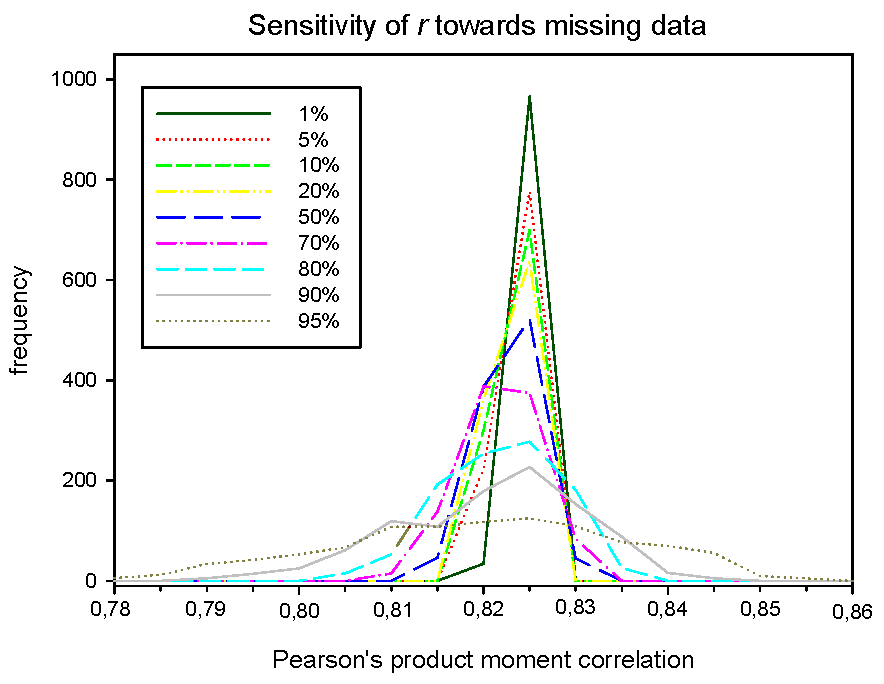
\includegraphics[width=0.75\textwidth]{Graphics/Simulation-MissingValues}
\end{figure}

It is possible to calculate the correlation matrix \arr{R} robustly towards missing values (see fig. \ref{fig:Miss}). However, the resulting matrix will no longer be positive definite and large eigenvalues will be overestimated, while small eigenvalues are underestimated. To be suitable for factor analysis or PCA, \arr{R} must be
\begin{description}
  \item[positive definite]{which means that \(\AbsVec{x}^T \arr{R} \AbsVec{x} > 0\enspace \forall\enspace \AbsVec{x} \) with at least one element \(\neq 0 \). A positive definite matrix has a determinant \(||\arr{R}|| > 0 \). In our case, \(||\arr{R}|| = \num{e-56} \approx 0 \). For a positive definite matrix all leading principal minors (the \skalar{i}-th \textbf{leading principal minor} of an \(n \times n \) matrix is the determinant of the submatrix containing its first \skalar{i} rows and its first \skalar{i} columns) are also positive (\Name{Sylvester}'s criterion). Computational errors may result in small positive or negative values instead of zero for semi-definite matrices.}
  \item[invertible]{No data column \skalar{i} may be a constant, as this would result in \(\arr{R}_{\cdot i} = \arr{R}_{i\cdot} = 0 \). No data column \skalar{i} can be replicated by a linear combination of any of the remaining \(p-1 \) columns, otherwise the \skalar{i}-th row and column of \arr{R} will be linear combinations of other columns or rows, respectively and therefore \(||\arr{R}|| = 0 \).}
\end{description}

\subsubsection{Shrinkage of \arr{S}}\label{text:shrinkage}

The \Name{Ledoit-Wolf}-procedure \parencite{Scha-05,Kwa-11,Led-03} tries to turn a semi-definite matrix into a definite  by ``shrinkage''. In effect, all eigenvalues are moved towards their grand mean, while maintaining the eigenvectors.

\paragraph{Weighted average of \arr{S} with another matrix}
For example, a \(\arr{B}_{p \times p} \) diagonal matrix with \(\arr{B}_{ii} = \arr{S}_{ii} \) the variances in the diagonal (that is, \(\arr{B} = \diag(\arr{S}) \)) is always positive definite, because \(\AbsVec{x}^T \arr{B} \AbsVec{x} = \sum_{j=1}^{p} \AbsVec{x}_j^2 \arr{B}_{jj} > 0 \) if there is at least one element \(\AbsVec{x}_j \neq 0 \). Then the weighted average of \arr{B} and \arr{S} is defined as \(\widehat{\arr{S}} = (1-\omega)\arr{S} + \omega \arr{B} \) with a weight \(0 < \omega < 1 \), and is always positive definite because \(\AbsVec{x}^T \widehat{\arr{S}} \AbsVec{x} = (1-\omega) \AbsVec{x}^T \arr{S} \AbsVec{x} + \omega \AbsVec{x}^T \arr{B} \AbsVec{x} > 0 \). If \(\omega = 0 \), then \(\widehat{\arr{S}} = \arr{S} \), and if \(\omega = 1 \), then \(\widehat{\arr{S}} = \arr{B} \).

\paragraph{Optimal \skalar{\omega}}
The covariances \(s_{ij}, i \neq j \) in \arr{S} are sample estimators of the population covariances \skalar{\sigma_{ij}}. Then \([(1-\omega) s_{ij} - \sigma_{ij}]^2 \) can be viewed as loss, and we would like to find the \(\omega \) that minimises \(\sum_{i=1}^p{\sum_{j=i+1}^{p}{[(1-\omega) s_{ij} - \sigma_{ij}]^2}} \) for all elements of the upper triangle of \arr{S} (of course, the lower triangle would give the same result because of symmetry) \parencite{Kwa-11}. Then
\begin{equation} \label{eqn:omegaW}
  \omega = \frac{\sum_{i=1}^p{\sum_{j=i+1}^{p}{\var(s_{ij})}}}{\sum_{i=1}^p{\sum_{j=i+1}^{p}{[\var(s_{ij}) + \sigma_{ij}^2]}}}
\end{equation}
We note that because the nominator is larger than the denominator and both are positive, the condition \(0 < \omega < 1 \) is met by necessity. To get \(\var(s_{ij}) \) we introduce for each pair of variables \(i,j = 1..p \)  a random variable \(\AbsVec{g}_{ij} \), which is the product of the centered data columns \(\AbsVec{X}_{\cdot{i}} \) and \(\AbsVec{X}_{\cdot{j}} \). Then \(\bar{\AbsVec{g}}_{i,j} = 1/n \sum_{k=1}^{n}{[(\AbsVec{X}_{k,i} - \bar{\AbsVec{x}}_i) (\AbsVec{X}_{k,j} - \bar{\AbsVec{x}}_j)]} \) and \(\var(s_{i,j}) = \frac{n}{(n-1)^3} \sum_{k=1}^n{(\AbsVec{g}_{kij} - \bar{\AbsVec{g}}_{i,j})^2} \) and \(E(s_{i,j}) = \sigma_{i,j} \) and hence \(\sigma_{ij}^2 = s_{i,j}^2 \) \skalar{\omega} can be calculated.

\paragraph{Non-linear shrinkage}
In the simplest case, shrinkage is done linearly by a certain factor \skalar{\omega} as discussed.  Nonlinear shrinkage has been shown to be at least as effective, and most of the time more, than linear \parencite{Led-17}. R package \texttt{nlshrink} provides this method. The method is described for \arr{S}, it is unclear how this would extend to \arr{R}.

\subsubsection{Shrinking a correlation matrix \arr{R}}

Under some simplifying assumptions, the basic idea is the same as with the variance-covariance matrix, but shrinkage is achieved by calculating a weighted average between \arr{R} and the identity matrix \arr{I} \parencite{Scha-05,Kwa-11}. Then equation \ref{eqn:omegaW} becomes
\begin{equation} \label{eqn:omegaR}
  \omega = \frac{\sum_{i=1}^p{\sum_{j=i+1}^{p}{\var(r_{ij})}}}{\sum_{i=1}^p{\sum_{j=i+1}^{p}{[\var(r_{ij}) + \rho_{ij}^2]}}}
\end{equation}
where \(\rho_{ij} \) is the population correlation coefficient of variables \skalar{ij}. \(\var(r_{ij}) = \frac{\var(s_{ij})}{s_{ii} s_{jj}} \) and \(\rho_{ij}^2 = \frac{s_{ij}^2}{s_{ii} s_{jj}} \). The R-package \texttt{corpcor} provides shrinkage for \arr{S} and \arr{R}.

\begin{figure}
   \caption{Effect of shrinkage (using \(\bar{\arr{R}} \)) on a correlation matrix that is not positive semi-definite. With increasing \(\omega \) the correlation coefficients move towards the common mean, the distribution becomes narrow and steep. An \(\omega = 0.5\ldots 0.6 \) is optimal with this matrix, further increases of \(\omega \) have no beneficial effect.}
   \label{fig:shrink1}
   \centering
      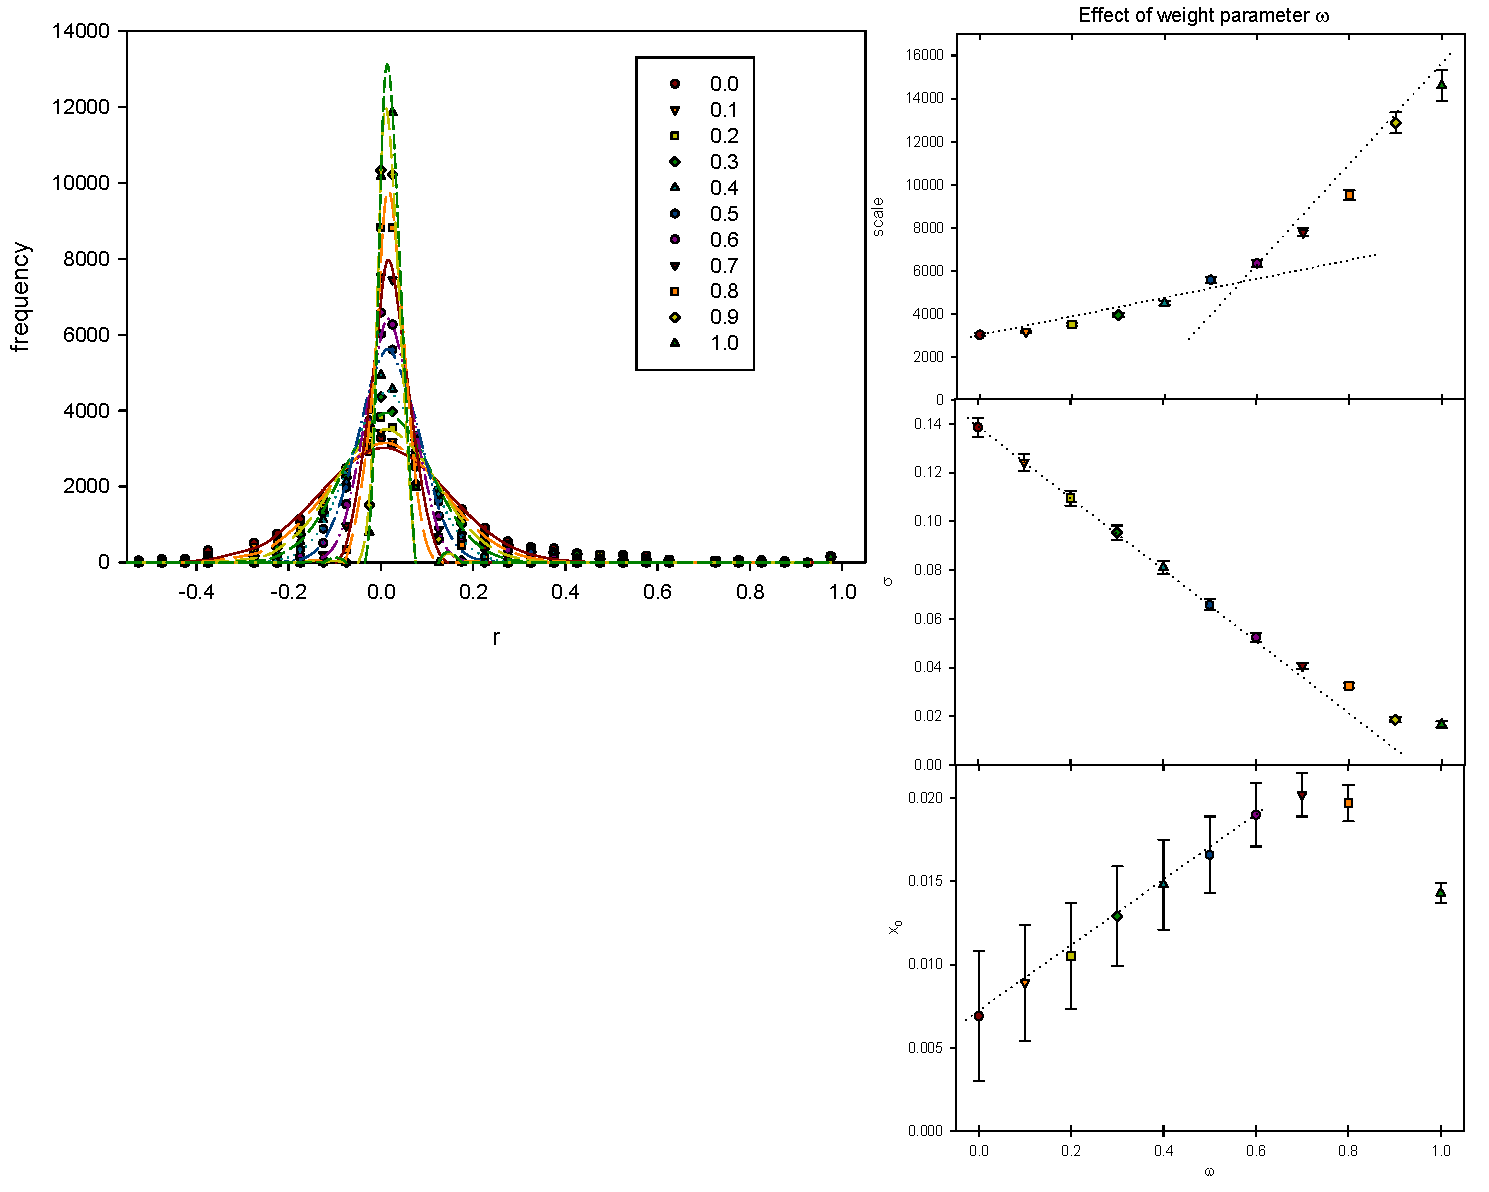
\includegraphics[width=\textwidth]{Graphics/Effect-omega-on-r}
\end{figure}

\begin{figure}
   \caption{Effect of shrinkage (using \(\bar{\arr{R}} \)) of a correlation matrix that is not positive semi-definite. With increasing \(\omega \) the number of positive eigenvalues increases, the maximum cumulative explained variance decreases. An \(\omega = 0.5\ldots 0.6 \) is optimal with this matrix, further increases of \(\omega \) have no beneficial effect. In the scree-plot the lines of different \(\omega \) intersect in a common point, this point is to the right of the number of valid components.}
   \label{fig:shrink2}
   \centering
      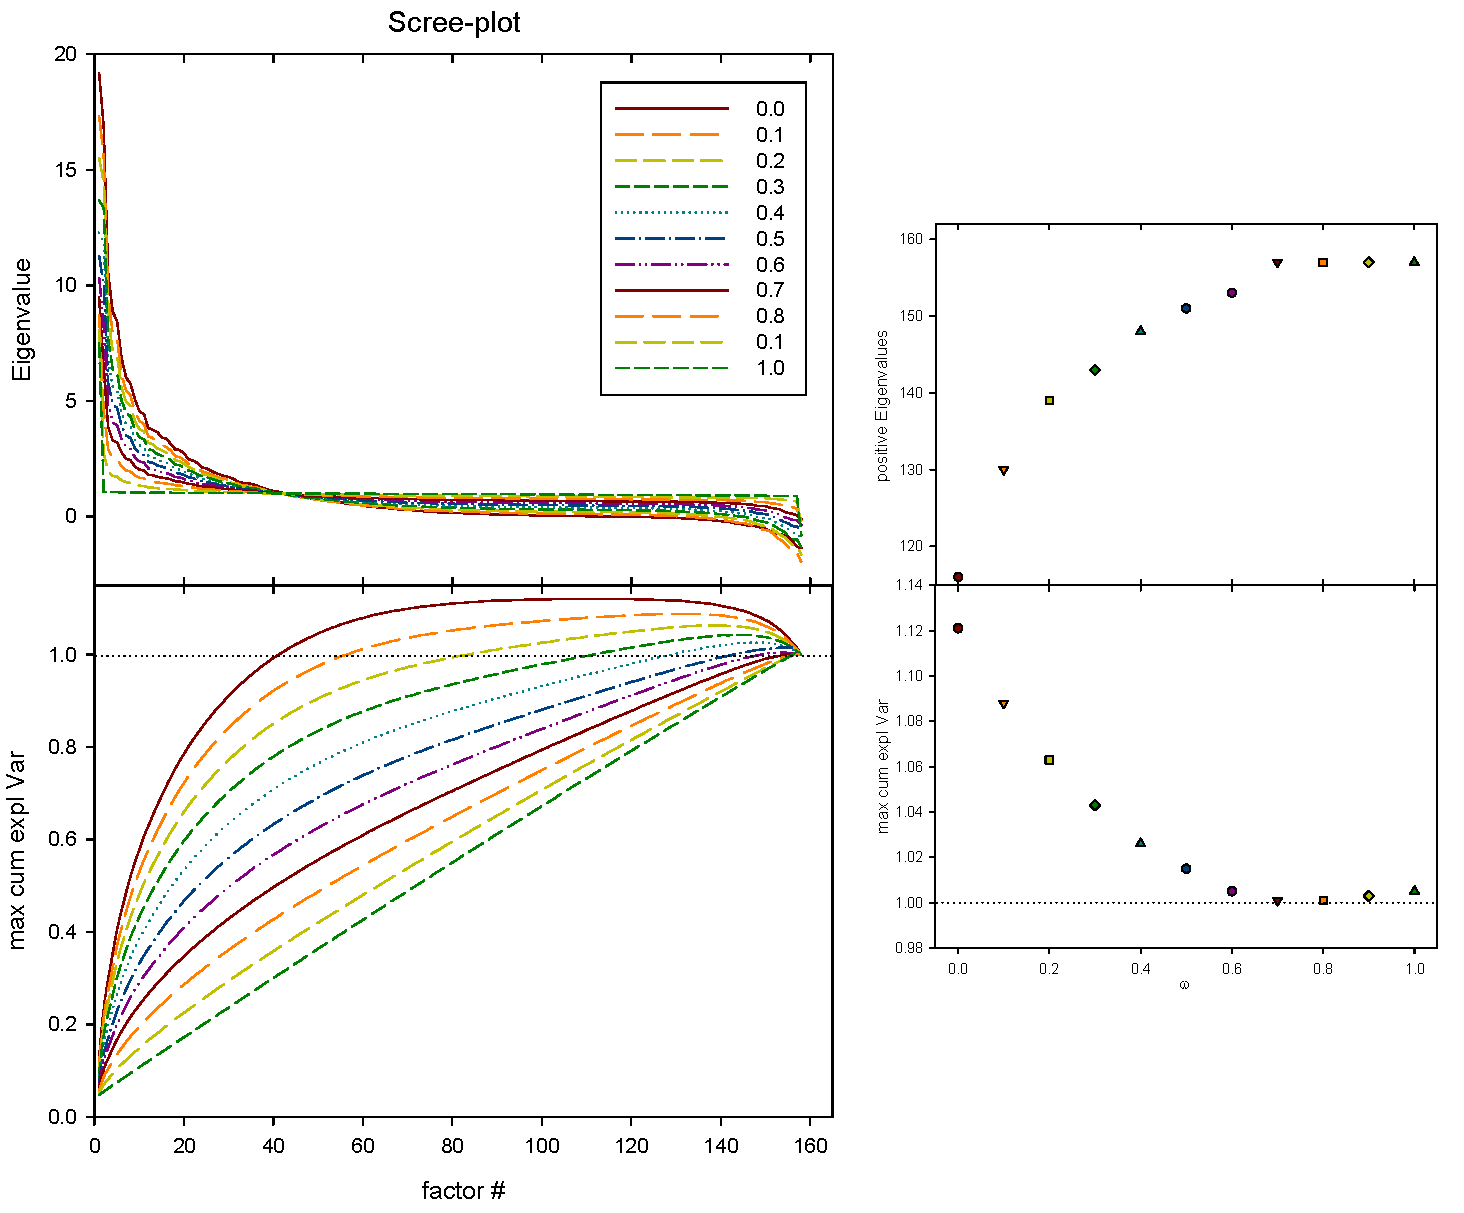
\includegraphics[width=\textwidth]{Graphics/Effect-omega-on-Scree}
\end{figure}

Alternative is to first calculate the average correlation of each variable with all others:
\begin{equation}
   \bar{\skalar{r}}_{i\cdot} = \frac{1}{p-1} \sum_{j=1}^p{\skalar{r}_{ij}} \enspace \forall \enspace j \neq i
\end{equation}
Then the correlation coefficient \(\hat{\skalar{r}}_{ij} = (\bar{\skalar{r}}_{i\cdot} + \bar{\skalar{r}}_{j\cdot}) /2 \) \parencite{Dis-07}. This matrix is positive definite and performs very similar to that described by \parencite{Kwa-11} with optimal \(\omega \) (see fig. \ref{fig:shrink1} and \ref{fig:shrink2}).

\paragraph{Recalculation of \arr{R} and \arr{S} from results of an initial eigenanalysis}

If the correlation matrix \arr{R} is indefinite and returns negative eigenvalues, these can be seen as experimental error (they are usually small). Hence, they are set to zero and a definite correlation matrix \(\widehat{\arr{R}} \) is produced from the corrected eigenvalue matrix \(\diag(\hat{\lambda}) = \hat{\Lambda} \) and the eigenvectors \arr{E} by
\begin{equation}
  \widehat{\arr{R}} = \arr{E} \hat{\Lambda}\ \arr{E}^{-1}
\end{equation}
Then the final eigenanalysis is performed on \(\widehat{\arr{R}} \) \parencite{TL-07}.

It was found, however, that the result of this procedure are \SI{0.5}{\%} correlation coefficients that are outside the range \([-1..+1] \), and many diagonal elements \(\neq +1 \). If this is corrected, negative eigenvalues return, but fewer than with the original correlation matrix. Hence this procedure can be repeated iteratively, until the number of illegal entries in the correlation matrix becomes zero.

\begin{lstlisting}[caption=Correction of non-definite correlation matrices]
  UNIT PerformShrinkage;

  INTERFACE

  USES Math, MathFunc, Vector, Matrix, EigenValues;

  PROCEDURE ErzeugeLambda(CONST Eigenvalues: VectorTyp; VAR Lambda: MatrixTyp);
  { Turn vector of eigenvalues into a diagonal matrix }

  PROCEDURE Average(VAR R: MatrixTyp; omega: double);
  { Shrink the correlation matrix R by calculating the weighted average between R
    and the row means of R for each i and j. omega (0..1) is the relative weight
    of of the average, the relative weight of R is (1-omega) }

  PROCEDURE Shrinkage(VAR R: MatrixTyp; omega: double);
  { Shrink the correlation matrix R by calculating the weighted average between R
    and the identity matrix. omega (0..1) is the relative weight of I, the relative
    weight of R is (1-omega) }

  PROCEDURE NormaliseCorrelations(VAR R: MatrixTyp);
  { make an indefinite correlation matrix positive definite for eigenanalysis,
    by setting all eigenvalues < 0 to zero and re-calculating R = E Lambda E^{-1}. }

  IMPLEMENTATION

  PROCEDURE ErzeugeLambda(CONST Eigenvalues: VectorTyp; VAR Lambda: MatrixTyp);

  VAR
    p, i, j: WORD;

  BEGIN
    p := VectorLength(Eigenvalues);
    CreateIdentityMatrix(Lambda, p);
    FOR j := 1 TO p DO
      SetMatrixElement(Lambda, j, j, GetVectorElement(Eigenvalues, j));
  END;


  PROCEDURE Average(VAR R: MatrixTyp; omega: double);

  VAR
    p, i, j: WORD;
    Averages: VectorTyp;
    Sum, w: double;

  BEGIN
    IF (omega < 0) OR (omega > 1)
      THEN
        BEGIN
          Writeln('Shrinkage: omega not in [0..1]');
          HALT;
        END;
    p := MatrixRows(R);
    CreateVector(Averages, p, 0);                // calculate row-averages OF R
    FOR i := 1 TO p DO
      BEGIN
        Sum := 0;
        FOR j := 1 TO p DO
          IF (i = j)
            THEN  // ignore correlation WITH self
            ELSE  Sum := Sum + GetMatrixElement(R, i, j);
        SetVectorElement(Averages, i, Sum / Pred(p));
      END;
    w := 1 - omega;
    omega := omega / 2;                               // weight FOR each r_i AND r_j
    FOR i := 1 TO p DO                              // calculate NEW elements OF R
      FOR j := Succ(i) TO p DO
        BEGIN
          Sum := (W * GetMatrixElement(R, i, j) + omega *
            GetVectorElement(Averages, i) + omega * GetVectorElement(Averages, j));
          SetMatrixElement(R, i, j, Sum);
          SetMatrixElement(R, j, i, Sum);
        END;
    DestroyVector(Averages);
  END;


  PROCEDURE Shrinkage(VAR R: MatrixTyp; omega: double);

  VAR
    p, i, j: WORD;
    Sum, w: double;

  BEGIN
    IF (omega < 0) OR (omega > 1)
      THEN
        BEGIN
          Writeln('Shrinkage: omega not in [0..1]');
          HALT;
        END;
    w := 1 - omega;
    p := MatrixRows(R);
    FOR i := 1 TO p DO                              // calculate NEW elements OF R
      FOR j := Succ(i) TO p DO
        BEGIN
          Sum := (W * GetMatrixElement(R, i, j)); // non-diagonal elements OF I are 0
          SetMatrixElement(R, i, j, Sum);        // AND can be ignored
          SetMatrixElement(R, j, i, Sum);
        END;
  END;


  PROCEDURE NormaliseCorrelations(VAR R: MatrixTyp);

  VAR
    Eigenvalues: VectorTyp;
    Eigenvectors, Hilfs, Lambda, RecipEV: MatrixTyp;
    i, iter, n, NoNegs, j: WORD;
    Rneu: double;

  BEGIN
    n := MatrixRows(R);
    Writeln('Initial calculation of eigenvalues');
    iter := 1;
    REPEAT
      INC(iter);
      i := Jacobi(R, Eigenvalues, Eigenvectors, j);  // eigenanalysis
      Write(iter: 2, ': ', j: 3, ' iterations, Result = ', i: 1);
      CASE i OF
        0    : Write(' ok             ');
        5    : Write(' no convergence ');
        ELSE   Write(' error          ');
      END;
      NoNegs := 0;
      FOR i := 1 TO n DO
      BEGIN
        IF (GetVectorElement(Eigenvalues, i) < 0)
          THEN
            BEGIN
              SetVectorElement(Eigenvalues, i, 0);
              INC(NoNegs);
            END;
      END;
      Writeln(NoNegs: 3);
      DestroyMatrix(R);
      ErzeugeLambda(Eigenvalues, Lambda);
      CopyMatrix(EigenVectors, RecipEV);
      InverseMatrix(RecipEV);
      MatrixInnerProduct(EigenVectors, Lambda, Hilfs);    // calculate R = E Lambda E^{-1}
      MatrixInnerProduct(Hilfs, RecipEV, R);
      DestroyMatrix(EigenVectors);
      DestroyMatrix(RecipEV);
      DestroyMatrix(Hilfs);
      DestroyMatrix(Lambda);
      DestroyVector(EigenValues);
      FOR i := 1 TO n DO
        BEGIN
          FOR j := 1 TO n DO
            BEGIN
              Rneu := GetMatrixElement(R, i, j);
              IF (Abs(Rneu) > 1.0)
                THEN SetMatrixElement(R, i, j, sign(Rneu));  // max + OR - 1
            END;
          SetMatrixElement(R, i, i, 1.0);                 // diagonal elements 1
        END;
    UNTIL (iter >= 100) OR (NoNegs = 0);
  END;

  END.
\end{lstlisting}

The various methods of shrinkage perform similarly in practice, so numerical simplicity can be the overriding selection criterium \parencite{Dis-07}. The one exception is the recalculation of \arr{R} and \arr{S} from initial eigenanalysis, which raises suspicion against that method.

\subsection{Effect of discrete variables on PCA}

Component analysis was originally developed for interval- and rational scaled variables with multivariate normal distribution. In \parencite{Kol-04} the effects of the use of ordinal and binary scaled, and/or non-normally distributed variables (skew and kurtosis) is investigated. If one assumes that categorial data are generated by quantising underlying cardinal data (with \( < 5 \) categories) the correlation coefficients will be biased towards 0 (their fig. 2). This will affect the principal component weights. Categorization can be viewed as a measurement error with nonlinear properties. Errors can be minimised if all categories have similar numbers of observation. \acs{PCA} is quite robust toward different distances between the categories of a variable.  On average, a discrete variable contains 2/3 of the information of the underlying cardinal variable.

Sometimes dummy variables corresponding to individual categories are used. \Foreign{E.g.}, an ordinal value for affluence may be mode of transport (walk, bicycle, motorcycle, car). One could replace this with four independent, binary variables (has car, has motorcycle...). However, the natural order of the variable, and hence information, would be lost. Also, the effect of quantisation is aggravated. Most weight is attached to the category with the highest number of observations. Also, \acs{PCA} becomes numerically less stable.

It is incorrect to use \Name{Pearson}'s correlation coefficient for nominal or ordinal data. The correlation coefficient between two variables is influenced by both their substantive similarity and by their statistical distributions. If the distributions are dissimilar, then \acs{FA} or \acs{PCA} may give a spurious multidimensional results. Polychoric correlations have been successfully tried with \Name{Likert}-scale data \parencite{Bas-12}.

\subsection{Number of components}

\acs{PCA} is used to reduce the dimensionality of the data set, this makes interpretation easier and removes random noise. It may also make further analysis (multiple regression, clustering) more stable by removing co-linearity. However, it also leads to a loss of information. The question therefore is how many components are significant enough to be included in the following analysis. In general, too many components cause fewer problems than too few \parencite{Bas-12}.

\subsubsection{Scree-plot}\label{text:scree}

\begin{figure}
   \caption{Example for a scree-plot, from an investigation on validity of exam questions. The two leftmost components form the mountain and are used for analysis, the remaining components are discarded as rubble. The acceleration is the second derivative of the scree-plot and can sometimes help to identify the ``knee''. Here, it would suggest that third eigenvalue may also be significant.}
   \label{fig:Scree}
   \centering
      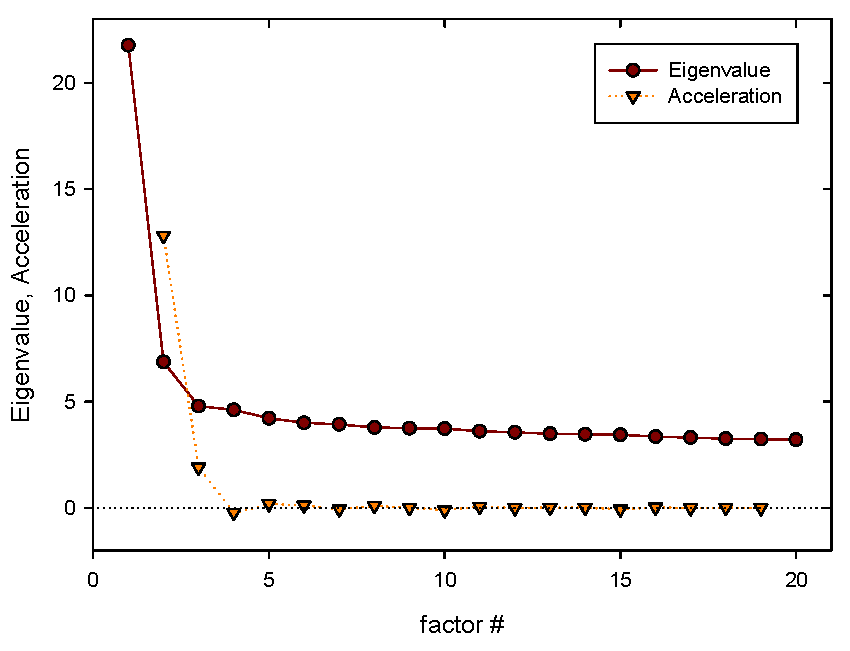
\includegraphics[width=0.75\textwidth]{Graphics/Acceleration}
\end{figure}

In a plot of eigenvalue vs factor or component number (see fig. \ref{fig:Scree}) \parencite{Cat-66} one sees initially a steep exponential decline (``cliff'') followed by a shallow area with linear decline (``rubble'' or ``scree''). The cliff (data left of the ``knee'') represents the significant components. However, distinguishing cliff and scree can be difficult and subjective. The \textbf{acceleration factor} is calculated as the second derivative of the scree-curve by finite differences, \(f''(j) \approx (f(j+1) - 2f(j) + f(j-1)) \), it should have a maximum at the knee. This is usually not discernible, but for non-significant components this value oscillates around zero.

\subsubsection{\Name{Kaiser}-criterion}

All components with an eigenvalue \(> \bar{\lambda} \) are considered significant. This average is \num{1.0} when a \skalar{z}-standardised data matrix is used (or when the eigenanalysis is performed on \arr{R} rather than \arr{S}), so the variance of each variable is \num{1.0}. The eigenvalue is the sum of the squared loadings of a component with all variables and corresponds to the variance explained by this component. However, in an analysis with many variables the \Name{Kaiser}-criterion overestimates the number of significant components, as some eigenvalues will be \(> 1 \) by chance (variables uncorrelated in the population have small correlation in the sample, leading to significant eigenvalues).

\subsubsection{Variance explained}

The retained components are supposed to retain the significant information of the data, but not the noise. One can simply set a minimal value for explained variance, say, \SI{5}{\%} or \SI{10}{\%}. Components that account for less are discarded. Alternatively, enough components are retained so that the cumulative explained variance is \num{70}--\SI{80}{\%}.

\subsubsection{Parallel analysis}

\acs{PCA} is performed both with the empirical data set and with (at least 100) data sets of random numbers (if data are normally distributed) or a permuted data set (if data have a non-normal distribution). The number of cases and variables in the random set should be identical  to the empirical. Only those eigenvalues in the empirical data are considered significant that are larger than those from the random data. Standard statistical packages do not include this computationally expensive method, so it is under-used.

\subsubsection{\Name{Bartlett}'s test for sphericity}

It is possible to use \Name{Bartlett}'s sphericity test to calculate the significance of the difference between eigenvalues. Say, we have a test with \(n = 100 \) persons and \(p = 3 \) variables. The eigenvalues are 8, 4, 2 \parencite{Hop-75}. Then according to eqn. \ref{eqn:Bart} \(r = 0.8571, r^3 = 0.6295, \chi^2 = 44.66 \) and \(f = 5 \), therefore \(P_0 < \SI{0.1}{\%} \). Next, we eliminate the first eigenvalue and calculate the test values for the remaining eigenvalues:
\begin{align}\label{eqn:BartNo}
   r      &= \frac{(4 \times 2)^{1/2}}{1/2 \times (4 + 2)} = \frac{\sqrt{8}}{3} \\
   r^2    &= \frac{8}{9} \notag \\
   \chi^2 &= -(100 - 3 - 1/2) (-0.11779) = 11.37 \notag \\
   f      &= \frac{(3 - 1 + 2) (3 - 1 -1)}{2} = 2 \notag
\end{align}
We then take the difference between both \(\chi^2 \)-values (44.66 - 11.37 = 33.29) and degrees of freedom (5 - 2 = 3) and use the result to test for the significance of the difference between the first and second eigenvalue (\( P_0 < \SI{0.1}{\%} \)). This process is continued until that difference becomes non-significant or until only one eigenvalue is left.

From this procedure we learn how many data are required to \emph{describe} the data, not necessarily how many can be used to \emph{describe} them. For singular correlation matrices \(\chi^2 \) will remain significant for all \skalar{p} components.

\subsubsection{Very simple structure (VSS)}

This method compares the original correlation matrix with that reproduced from the retained eigenvalues and -vectors \parencite{Rev-79}. As the number of retained components increases, VSS index increases sharply to a maximum, then decreases slowly. Procedure:
\begin{enumerate}
  \item{Extract components by the method of your choice, and make an initial estimate of the number of relevant components \skalar{q}}
  \item{Rotate the components by the method of your choice, resulting in a rotated component matrix \(\arr{B}_{p \times q} \)}
  \item{Calculate VSS:
    \begin{enumerate}
      \item{For a VSS of complexity \skalar{v}, replace the smallest \(q-v \) elements of \arr{B} by zero, resulting in a degraded component matrix \(\arr{B}_{p \times q}' \)}
      \item{Calculate the degraded correlation matrix \(\arr{R}' = \arr{B}' \Lambda \arr{B}'^{-1} \)}
      \item{calculate the mean square residual \skalar{M} of both \arr{R} and \arr{R}' and \(\mathrm{VSS}_{v,p} = 1 - \frac{M_{\arr{R}'}}{M_\arr{R}} \)}
    \end{enumerate} }
  \item{Repeat this for all \skalar{q} from 1 to the rank of the matrix and plot the results against \skalar{q}}
\end{enumerate}

\subsubsection{\Name{Velicer}'s minimum average partial (MAP) criterium}
\parencite{Vel-76}. The test has been revised with the partial correlations raised to the 4th power
(rather than squared). Source code is available under \href{https://people.ok.ubc.ca/brioconn/nfactors/nfactors.html}{https://people.ok.ubc.ca/brioconn/ nfactors/nfactors.html} and in the R-package \texttt{paramap}.

\subsubsection{Extrapolation}

One can draw a line between the \skalar{p}-th eigenvalue and the \skalar{i+1}-th. Then one can estimate the \skalar{i}-th eigenvalue by extrapolation. Measured eigenvalues are considered relevant if they are significant larger than the estimated one. This method is used by the R-module \texttt{nFactors}.

\subsubsection{Newer methods}

\Name{Gavish \& Donoho} \parencite{Gav-14} have shown that for a data matrix which is large compared to its rank, the optimal number of singular values to retain is \(\omega\tilde{\sigma} \), where \skalar{\tilde{\sigma}} is the median of the singular values. For \skalar{n \times p} matrices, \skalar{\omega} depends on \(\beta = p / n \) as \(\omega(\beta) \approx 0.56\beta^3 - 0.95\beta^2 + 1.82\beta + 1.43 \).

\Name{Minka} \parencite{Min-00} uses \Name{Bayes}ian statistics to derive a probability function that reaches its highest value at the optimal number of components
\begin{eqnarray}
   \nonumber
   \hat{v}      =& \frac{\sum_{j=q+1}^p{\lambda_j}}{p-q} \\
   \nonumber
   m            =& pq - \frac{q(q+1)}{2} \\
   P(\arr{X}|q) =& \left(\prod_{j=1}^q{\lambda_i}\right)^{-n/2} \hat{v}^{-n(q-q)/2} n^{-(m+q)/2}
\end{eqnarray}
where \skalar{\hat{v}} is the average of the left-out eigenvalues, that is, the maximum-likelihood noise variance.

\subsubsection{Importance of minor components}

Components that explain only a small percentage of the variance of the population as a whole may explain a large part of the variance of a small number of persons. For example, in a psychiatric test the answer to the question ``Did somebody ever try to murder you?'' will be ``no'' for the vast majority of subjects. A component loading on this question therefore might be dropped as noise. However, for the few people who answer ``yes'', the discriminatory value of that question might be quite high. It can therefore be useful to look for individuals that score high on such minor components.

